\documentclass[aspectratio=169, handout]{beamer}
% \documentclass[aspectratio=169]{beamer}
\usetheme{boxes}
\usecolortheme{seagull}

\setlength{\parskip}{\medskipamount} 
\setlength{\itemsep}{10pt}
\setbeamersize{text margin left=15mm,text margin right=15mm} 
\setbeamertemplate{footline}[frame number]

\usepackage{hyperref}
\hypersetup{
    colorlinks=true,
    linkcolor=blue,
    filecolor=magenta,      
    urlcolor=cyan,
    citecolor=teal,
}

\usepackage[style=authoryear]{biblatex}
\addbibresource{refs.bib}
\AtBeginBibliography{\footnotesize}

% Title %%%%%%%%%%%%%%%%%%%%%%%%%%%%%%%%%%%%%%%%%%%%%%%%%%%%%
\title{(ADA) Texture representation in the visual processing hierarchy}
\author{Al Xin, axin@andrew.cmu.edu}
\institute{Rob Kass (Stats and PNC), Jenelle Feather (Psych and NI)}
\date{August 25, 2026} 

% Symbols %%%%%%%%%%%%%%%%%%%%%%%%%%%%%%%%%%%%%%%%%%%%%%%%%%%%%

\usepackage{amsthm}
\usepackage{amsmath}
\usepackage{amssymb}
\usepackage{amsfonts}

% New commands %%%%%%%%%%%%%%%%%%%%%%%%%%%%%%%%%%%%%%%%%%%%%%%%

% General mathematical symbols
% argmin help from egreg from tex.stackexchange.com/questions/5223
\newcommand{\R}{\mathbb{R}}
\newcommand{\onedim}{\mathbb{R}}
\newcommand{\ddim}{\mathbb{R}^d}
\newcommand{\kdim}{\mathbb{R}^k}

\newcommand{\eps}{\varepsilon}
\newcommand{\seq}[1]{\{ #1_{n} \}}
\newcommand{\bfs}[1]{\boldsymbol{ #1 }}

\DeclareMathOperator*{\sign}{sign}
\DeclareMathOperator*{\argmin}{arg\,min}
\DeclareMathOperator*{\argmax}{arg\,max}
\DeclareMathOperator*{\dist}{dist}
\DeclareMathOperator*{\diag}{diag}

% boldface
\newcommand{\bfX}{\mathbf{X}}
\newcommand{\bfx}{\mathbf{x}}
\newcommand{\bfY}{\mathbf{Y}}
\newcommand{\bfy}{\mathbf{y}}
\newcommand{\bfZ}{\mathbf{Z}}
\newcommand{\bfz}{\mathbf{z}}

% Sets
\newcommand{\setA}{\mathcal{A}}
\newcommand{\setB}{\mathcal{B}}
\newcommand{\setC}{\mathcal{C}}
\newcommand{\setF}{\mathcal{F}}
\newcommand{\rademacher}{\mathcal{R}}
\newcommand{\setP}{\mathcal{P}}

% General stats
\newcommand{\E}{\mathbb{E}}
\DeclareMathOperator*{\var}{Var}
\DeclareMathOperator*{\cor}{Corr}
\DeclareMathOperator*{\cov}{Cov}
\newcommand{\prob}{\mathbb{P}}

\newcommand{\indep}{\perp \!\!\! \perp}
\newcommand{\depen}{\cancel{\indep}}
\newcommand{\indic}{\mathbbm{1}}
\newcommand{\Xbar}{\overline{X}_n}
\newcommand{\Xsqbar}{\overline{X^2_n}}
\newcommand{\Xbarsq}{\overline{X}^2_n}
\newcommand{\Ybar}{\overline{Y}_n}
\newcommand{\lik}{\mathcal{L}}
\newcommand{\ton}[1]{#1_1, \dots, #1_n}
\newcommand{\fisher}{\mathcal{I}}
\newcommand{\sumn}{\sum_{i = 1}^n}
\newcommand{\prodn}{\prod_{i = 1}^n}

% Distributions
\newcommand{\hpp}{\textrm{HPP}}
\newcommand{\ipp}{\textrm{IPP}}
\newcommand{\geom}{\textrm{Geom}}
\newcommand{\iid}{\overset{\textrm{i.i.d.}}{\sim}}
\newcommand{\pois}{\textrm{Pois}}
\newcommand{\bern}{\textrm{Bern}}
\newcommand{\N}{\mathcal{N}}
\newcommand{\MVN}{\textrm{MVN}}
\newcommand{\unif}{\textrm{Unif}}
\newcommand{\binomial}{\textrm{Binom}}
\newcommand{\expo}{\textrm{Expo}}
\newcommand{\hgeom}{\textrm{HGeom}}


\begin{document}

\begin{frame}
\titlepage
\end{frame}

\begin{frame}{Argument outline (1/3)}
\small
\begin{itemize}
    \item In object recognition, image information is first processed in the primary visual cortex (V1), then passes through V2, V4, and the inferotemporal cortex (IT). 
    \item Later visual regions select for ``higher-level'' features. Outside of V1, the nature of these features remains ill-defined. 
    \item To identify these features, one can first propose a parameterization of visual images, then record neural responses to stimuli that vary across those parameters.   
    \item For instance, natural textures (e.g., sand, tree bark, etc.) can be separated into families based on \( N \)th-order joint image densities. Higher between-family separability indicates that the recorded neurons select for the \(N\)th-order statistics that parameterize unique families. 
    \item Previous work found better separability of texture families in V2 and V4 compared to V1. However, researchers disagree as to whether texture statistics remain well-encoded in IT. 
\end{itemize}
\end{frame}

\begin{frame}{Argument outline (2/3)}
\small 
\begin{itemize}
    \item Previous analysis found texture family separability to be lower in IT compared to V4. However, differences in the sparsity and reliability of neural firings impedes direct comparison between regions. 
    \item IT tends to be sparser in both within-site responses and population responses. That is, individual neurons respond to only a few stimuli, and stimuli tend to evoke responses from only a few neurons. 
    \item Sparse sites in IT could still be reliable (consistent responses to repeats of the same stimulus). In contrast, in non-IT regions, high sparsity corresponded to unreliability. 
    \item When correcting for reliability, we find that texture family separability consistently increases with each higher level region and that IT separability exceeds V4.
\end{itemize}
\end{frame}

\begin{frame}{Argument outline (3/3)}
\small 
\begin{itemize}
    \item Our results indicate that ``lower-level'' image features remain encoded in IT responses. That is, IT exhibits a sparse, ``efficient'' encoding of image features without necessarily summarizing over lower order statistics.
    \item Given the regional differences in sparsity and reliability, prior methods may have overestimated the reliability of IT sites and underestimated the separability in IT.
    \item Site sparsity and reliability might also be related to the effective dimensionality of the neural responses, which might be an avenue for further work.
    \item Sparseness in IT makes it difficult to determine whether unreliable sites indicate non-response to texture stimuli specifically or reflect general measurement error. Future work could experiment with a broader stimuli set to better explore the distribution of population sparsity.  
\end{itemize}
\end{frame}

\begin{frame}{Hierarchy of visual processing for object recognition}
\centering
\includegraphics[width=0.9\textwidth]{figures/eshuijs2023-visual_hierarchy.jpg}

{\small Figure sourced from \cite{eshuijs_m31_2023}}
\end{frame}

\begin{frame}{Visual texture perception}
\centering
    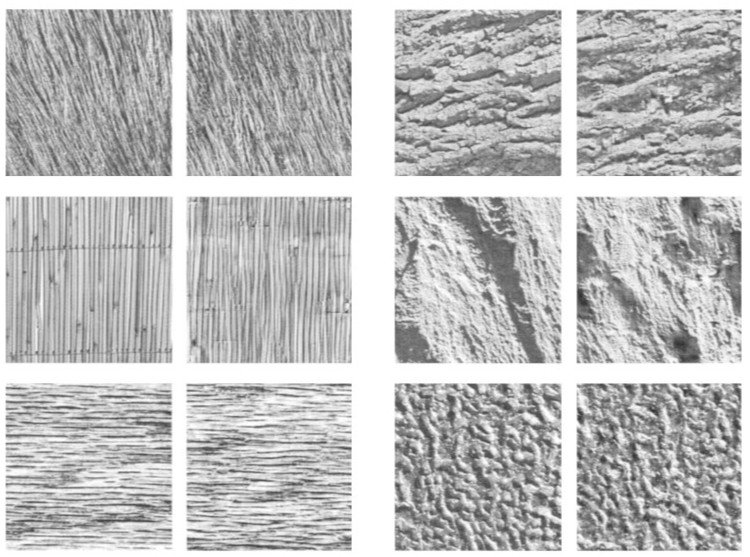
\includegraphics[width=0.6\textwidth]{figures/portilla_simoncelli2000-textures.jpg}
    
    {\small Example natural textures (Fig. 15 in \cite{portilla_parametric_2000}). For each pair, the left image was used as a seed to generate the statistics-matched images on the right.}
\end{frame}

\begin{frame}{Texture family separability increases along the visual hierarchy}
\centering
    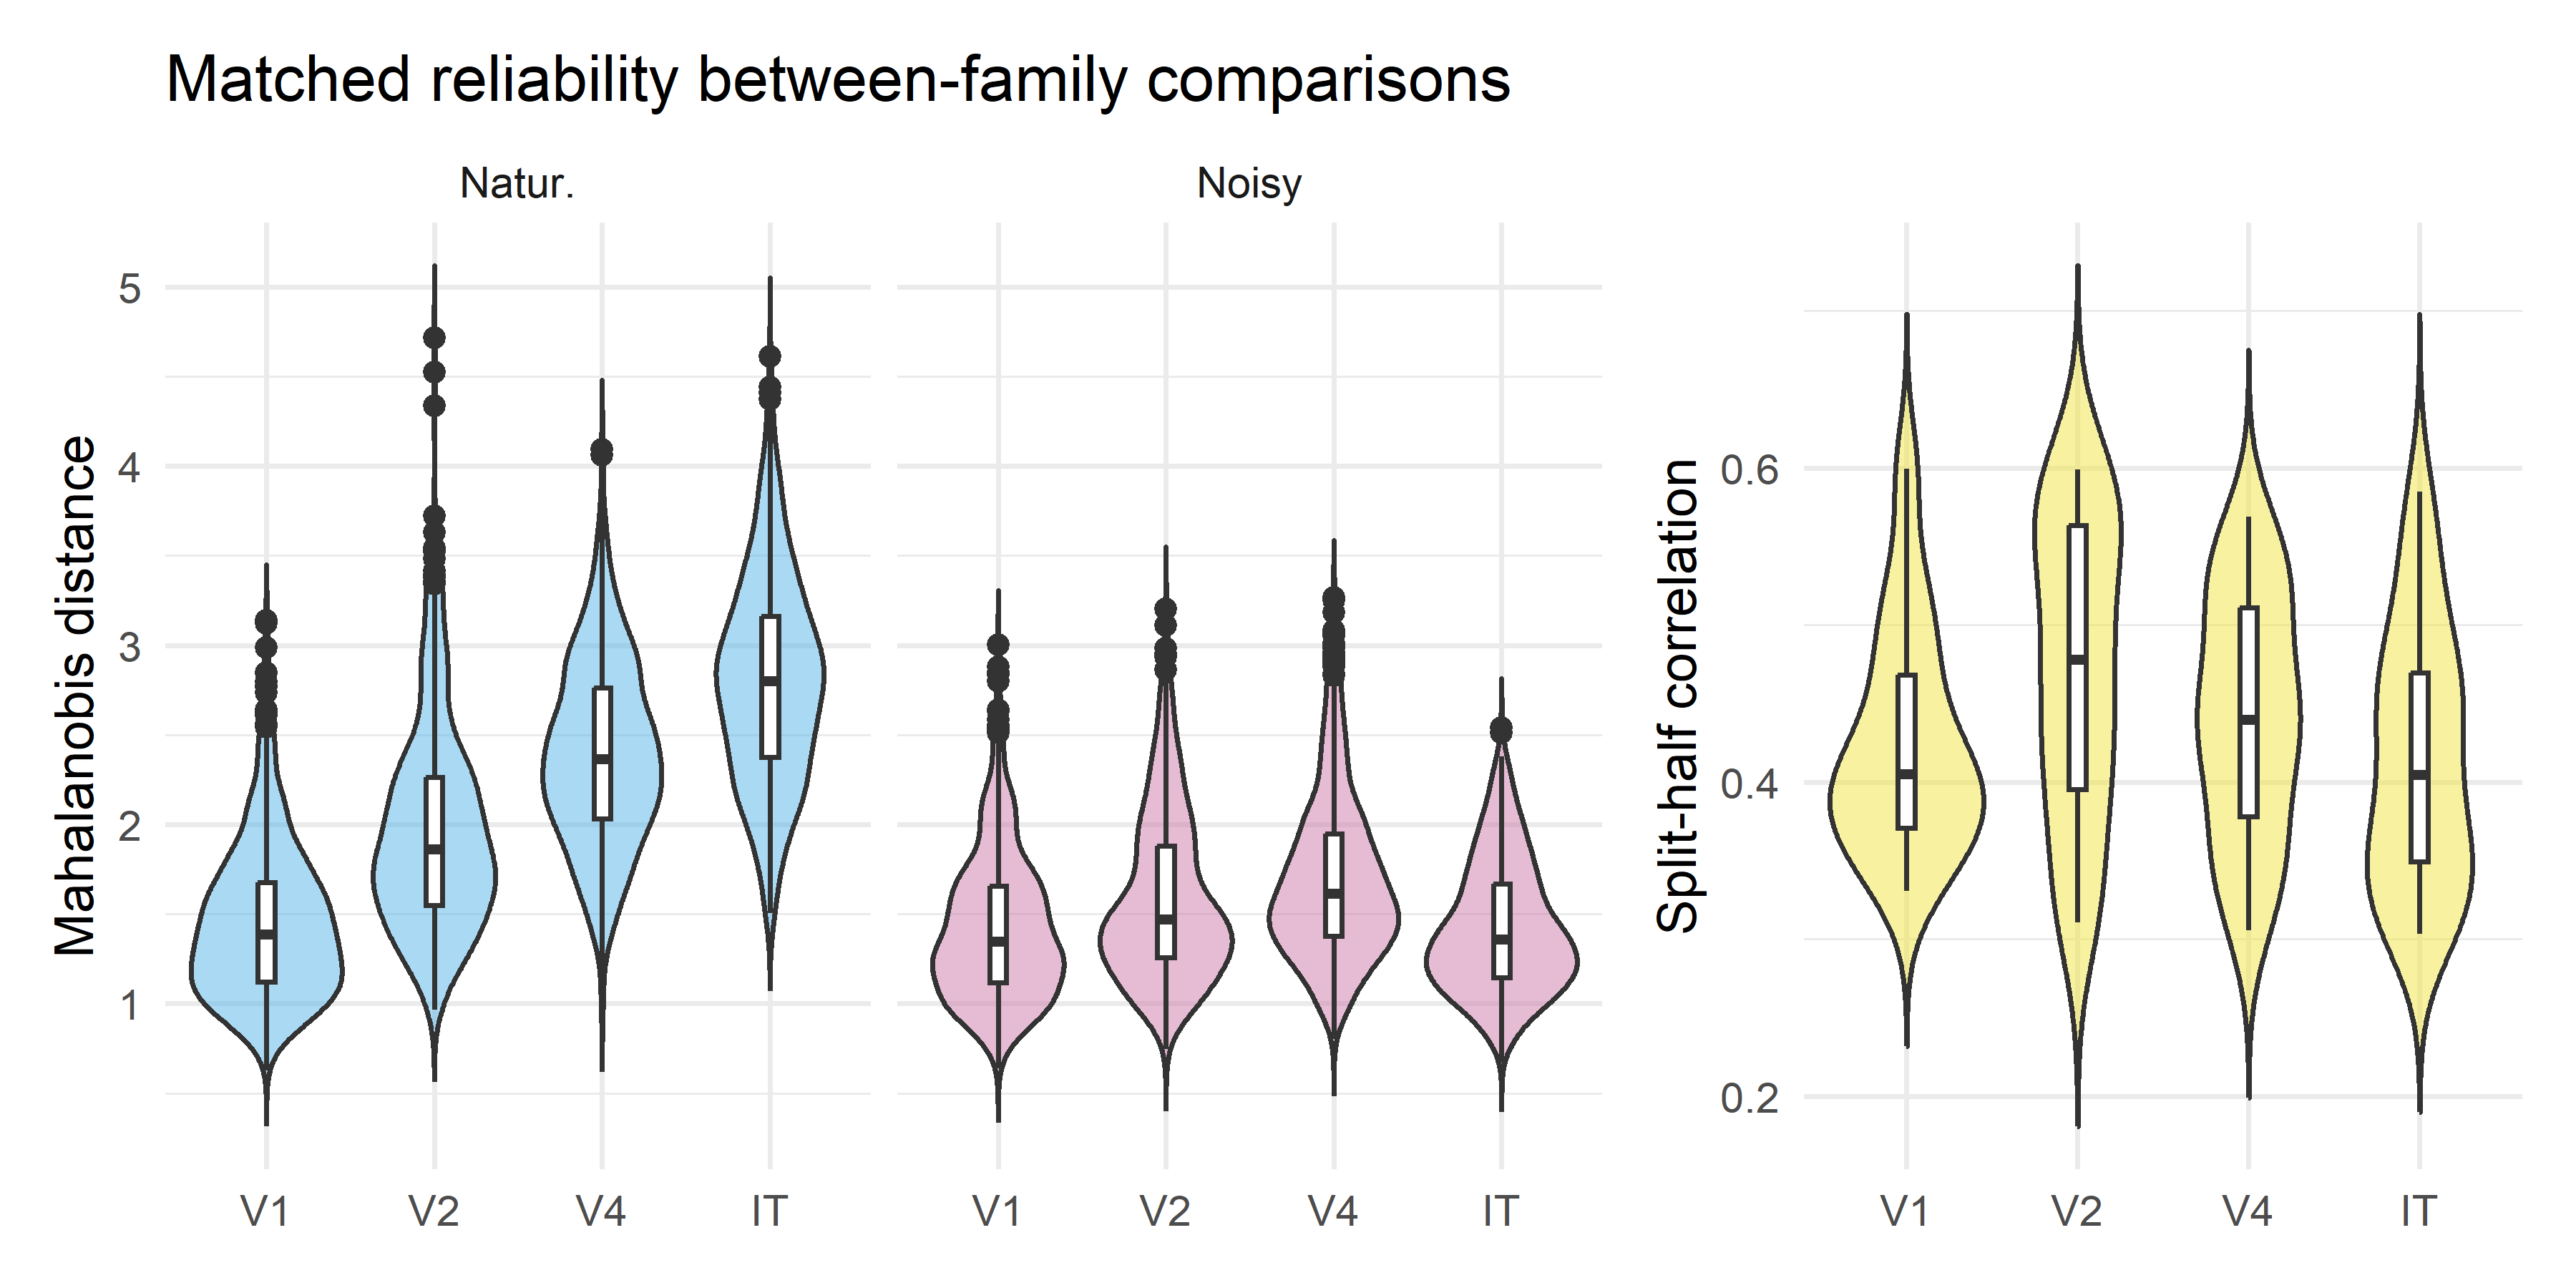
\includegraphics[width=0.9\textwidth]{figures/dM_pf.png}
    
    {\small (Left) Violin plots of the pairwise between-family Mahalanobis distances. Noisy stimuli lack higher \( N \)th-order statistics and show no clear trend.}

    {\small (Right) Reliability matching remains imperfect.}
\end{frame}

\section{Bibliography}
\begin{frame}[allowframebreaks]
\printbibliography
\end{frame}

\end{document}

\begin{frame}{Additional slides}
\end{frame}

\begin{frame}{Pointwise and joint confidence interval construction}

\end{frame}

\begin{frame}{Simulation results}
\end{frame}

\begin{frame}{Extension to generalized linear mixed models}
\begin{itemize}
    \item There is no analytic form for the pointwise and joint CIs. 
\end{itemize}
\end{frame}